\documentclass[11pt]{article}

\usepackage[margin=1in]{geometry}
\usepackage{graphicx}
\usepackage{booktabs}
\usepackage{caption}
\usepackage{authblk}
\usepackage{lineno}
\usepackage[numbers,super,sort&compress]{natbib}
\usepackage{hyperref}
\usepackage{microtype}

\hypersetup{
  colorlinks=true,
  linkcolor=black,
  citecolor=black,
  urlcolor=black
}

\linenumbers

\title{\bfseries Background matching audits mass spectral antimicrobial resistance prediction}

\author[1]{Byung Kim}
\author[2]{Collaborator Name}
\affil[1]{Department or Program, Institution, City, Country}
\affil[2]{Department or Program, Institution, City, Country}
\date{}

\begin{document}
\maketitle

\begin{abstract}
Machine-learning models trained on matrix-assisted laser desorption/ionization time-of-flight (MALDI-TOF) mass spectra can predict antimicrobial resistance, but external performance may reflect the bacteria that carry resistance rather than focal resistance biology alone. We introduce a model-agnostic background-matched audit that asks whether isolate-level predictions survive after matching samples by their co-resistance background. In an expanded \textit{Escherichia coli} DRIAMS panel, ciprofloxacin predictions retained within-background discrimination across temporal and external sites (background-centered AUC 0.703, 0.646 and 0.596 at A-2018, DRIAMS-C and DRIAMS-D), whereas amoxicillin-clavulanic acid weakened or collapsed toward chance (0.541, 0.497 and 0.486). The same audit applied to convolutional neural network and multi-task LightGBM outputs showed related attenuation, indicating that background sensitivity is not a single-architecture artifact. Cross-resistance networks revealed strong label blocks, including ciprofloxacin/norfloxacin (phi=0.976) and cephalosporin edges (phi=0.804--0.884). Public WGS-linked Bruker data further showed stronger MALDI encoding of ST131 lineage (AUC 0.906) than ciprofloxacin or ceftriaxone resistance. Background-matched evaluation therefore provides a practical guardrail for interpreting and deploying MALDI-TOF AMR models.
\end{abstract}

\section*{Introduction}

Rapid antimicrobial susceptibility testing remains a central bottleneck in the clinical management of bacterial infection. MALDI-TOF mass spectrometry is already embedded in clinical microbiology laboratories for organism identification, and this has motivated a large body of work asking whether the same spectra can also predict antimicrobial resistance (AMR). The DRIAMS resource established that MALDI-TOF AMR models can achieve useful performance across many organism-drug pairs and sites when trained and evaluated carefully\cite{weis2022driams,driamsdryad}. However, the biological interpretation of a successful MALDI-TOF AMR model remains unsettled.

The common performance question is simple: can a model predict resistance? The harder deployment question is different: what did the model learn, and will that signal remain valid at a different hospital? A resistant label is not an isolated molecular state. In bacterial populations, resistance is often carried by lineages, plasmid backgrounds, co-resistance blocks and hospital-specific ecological mixtures. Recent work in genomic AMR prediction has emphasized that population structure can confound machine-learning models by allowing phylogenetic markers to stand in for causal resistance markers\cite{yu2025population}. A MALDI-TOF model has the same vulnerability, because routine clinical spectra encode abundant cellular proteins and lineage-associated peak patterns. Prior MALDI-TOF AMR work has discussed phylogenetic structure as a confounder, and one preprint used hierarchical spectral stratification to alter evaluation splits\cite{weis2022stratification}. What is still missing is a practical, model-agnostic way to quantify how much of a MALDI-TOF AMR model's performance survives after resistant-population background is controlled.

Here we develop a Background-Matched MALDI-AMR Audit. The method takes isolate-level predictions from any model and asks whether the score for a focal drug still separates resistant from susceptible isolates after matching on the AST labels of the other drugs. This is deliberately modest: it does not prove the causal protein or clone behind a score. Instead, it supplies a stricter evaluation layer between raw external AUC and biological interpretation. If performance collapses inside matched co-resistance backgrounds, the original AUC was likely driven partly by resistant-population background. If performance survives, the model may contain a more focal or portable signal.

We apply this audit to DRIAMS-trained convolutional neural network (CNN) and LightGBM models, an expanded \textit{E. coli} drug panel, a cross-resistance network, and public WGS-linked Bruker MALDI data from a Basel uropathogenic \textit{E. coli} cohort\cite{cuenod2023papgii}. The resulting paper is not a claim that MALDI-TOF AMR prediction is impossible or useless. It is a framework for deciding when a reported AUC is likely to represent a portable focal-drug signal versus the spectral structure of the resistant bacterial population.

\section*{Results}

\subsection*{A model-agnostic audit for resistant-population background}

The audit begins with a long prediction table containing isolate identifier, site, year, organism, focal drug, true AST label and model probability. For each focal drug, we build a co-resistance background signature from the AST labels of the other drugs in the panel. We then retain only strata containing at least three resistant and three susceptible isolates for the focal drug. Three quantities are reported. Raw AUC measures ordinary external performance. Matched AUC measures performance only in valid co-resistance strata. Background-centered AUC subtracts each stratum's mean model score before pooling and recomputing AUC, thereby testing whether within-stratum ranking remains after removing the stratum-level background shift (Fig.~\ref{fig:framework}). Matched retention records how much of the original comparison remains interpretable.

\begin{figure}[ht]
\centering
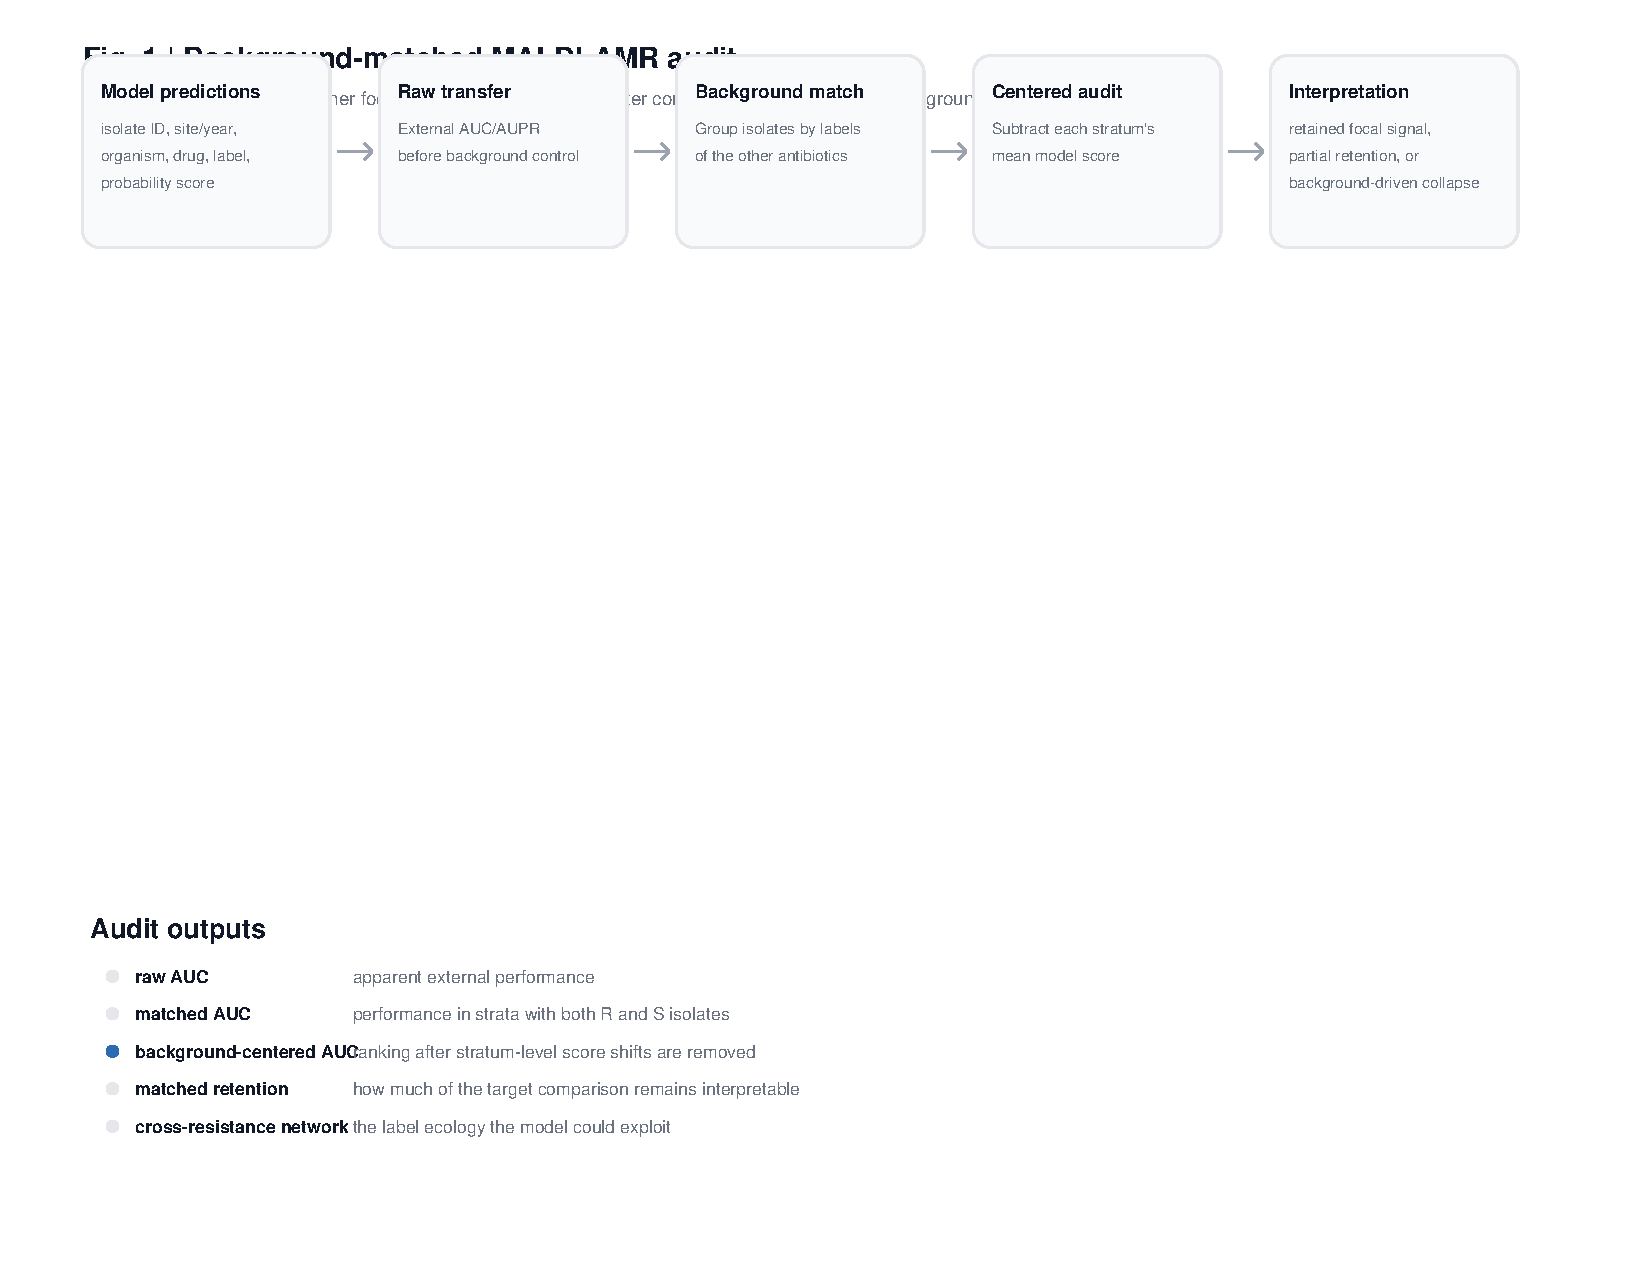
\includegraphics[width=\linewidth]{figures/figure_1_framework.pdf}
\caption{\textbf{Background-matched audit design.} The audit operates on isolate-level prediction rows from any MALDI-TOF AMR model. Co-resistance signatures are constructed from non-focal drug labels, valid strata are retained, and AUC is recomputed after centering scores within each stratum. The output distinguishes apparent raw transfer from residual within-background discrimination.}
\label{fig:framework}
\end{figure}

\subsection*{Ciprofloxacin retains more within-background signal than amoxicillin-clavulanic acid}

The main contrast compares \textit{E. coli}/ciprofloxacin with \textit{E. coli}/amoxicillin-clavulanic acid. This contrast is useful because the organism and training pipeline are shared, but the resistance ecology differs. Ciprofloxacin resistance in \textit{E. coli} is often embedded in globally disseminated fluoroquinolone-resistant lineages, including ST131\cite{nicolas2014st131}. Amoxicillin-clavulanic acid resistance is more heterogeneous and can reflect multiple beta-lactamase, inhibitor-resistance and background contexts.

Raw external AUC for ciprofloxacin was 0.823 in the temporal A-2018 split, 0.750 in DRIAMS-C and 0.671 in DRIAMS-D. After background centering, ciprofloxacin retained residual discrimination: 0.703, 0.646 and 0.596, respectively. DRIAMS-B gave a high centered estimate but with low matched support and is therefore treated as cautionary rather than primary evidence. In contrast, amoxicillin-clavulanic acid weakened substantially after matching. At DRIAMS-C and DRIAMS-D, centered AUCs were 0.497 and 0.486, despite high matched retention, consistent with collapse to chance inside co-resistance backgrounds. At A-2018 and DRIAMS-B, centered AUCs were 0.541 and 0.576, indicating weak or uncertain residual signal rather than robust focal discrimination (Fig.~\ref{fig:primary-audit}; Table~\ref{tab:primary-audit}).

\begin{figure}[ht]
\centering
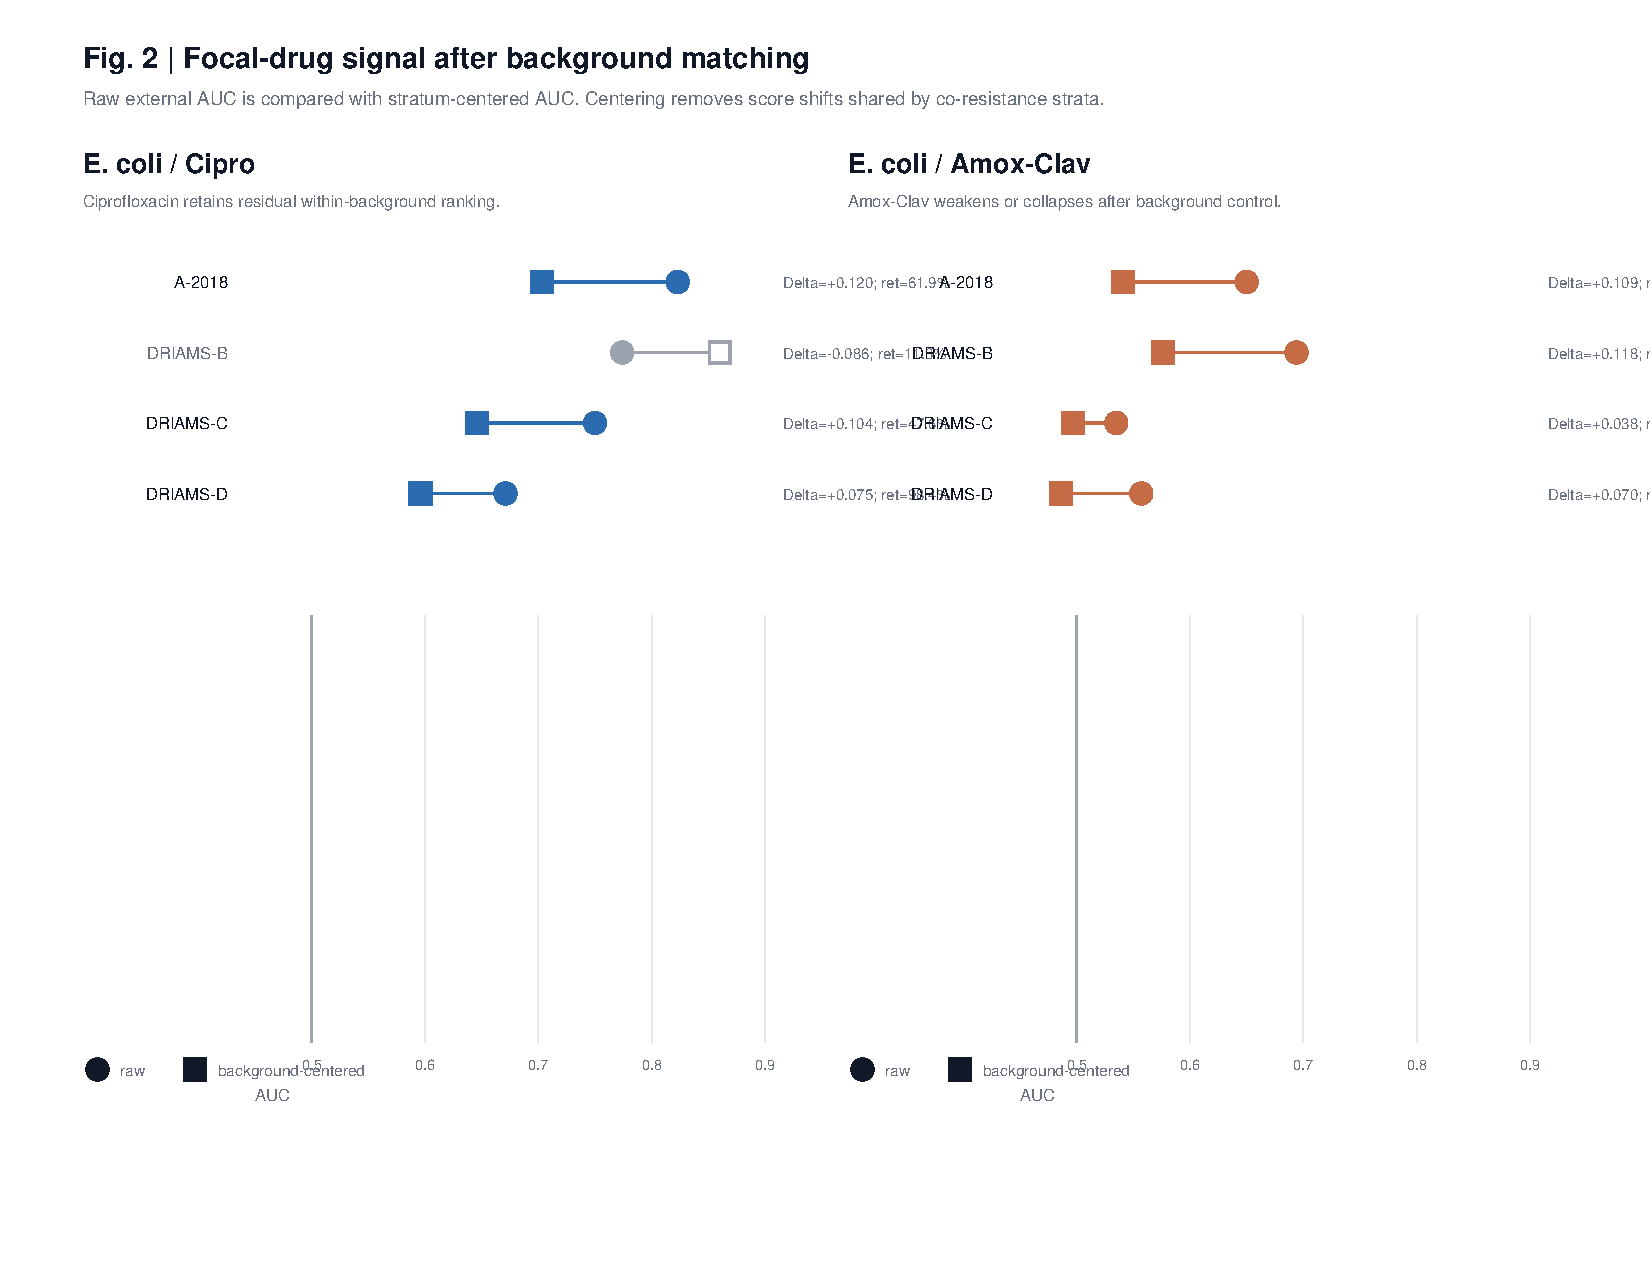
\includegraphics[width=\linewidth]{figures/figure_2_primary_background_audit.pdf}
\caption{\textbf{Raw external AUC versus background-centered AUC for the primary \textit{E. coli} contrast.} Circles show raw external AUC and squares show stratum-centered AUC after matching by co-resistance background. Ciprofloxacin retains more within-background signal than amoxicillin-clavulanic acid. Caution rows have low matched support and are not used as the main evidence.}
\label{fig:primary-audit}
\end{figure}

\begin{table}[ht]
\centering
\small
\caption{Primary background-matched audit for the E. coli ciprofloxacin and amoxicillin-clavulanic acid contrast.}
\label{tab:primary-audit}
\resizebox{\linewidth}{!}{%
\begin{tabular}{lccccccccc}
\toprule
Pair & Site & Raw AUC & Centered AUC & Pairwise acc. & Retention (\%) & n matched & P perm & Adequacy & Interpretation \\
\midrule
E. coli / Cipro & A-2018 & 0.823 (0.799-0.849) & 0.703 (0.664-0.747) & 0.754 & 61.9 & 836 & 0.002 & interpretable & Retained residual signal \\
E. coli / Cipro & DRIAMS-B & 0.774 (0.692-0.841) & 0.860 (0.636-1.000) & 0.860 & 11.8 & 25 & 0.010 & caution\_low\_n\_matched & Caution; low matched support \\
E. coli / Cipro & DRIAMS-C & 0.750 (0.702-0.795) & 0.646 (0.576-0.719) & 0.675 & 47.6 & 422 & 0.002 & interpretable & Retained residual signal \\
E. coli / Cipro & DRIAMS-D & 0.671 (0.640-0.700) & 0.596 (0.565-0.624) & 0.616 & 98.4 & 1908 & 0.002 & interpretable & Retained residual signal \\
E. coli / Amox-Clav & A-2018 & 0.650 (0.619-0.685) & 0.541 (0.504-0.576) & 0.546 & 92.2 & 1261 & 0.038 & interpretable & Weak or uncertain residual signal \\
E. coli / Amox-Clav & DRIAMS-B & 0.694 (0.611-0.765) & 0.576 (0.410-0.715) & 0.576 & 62.1 & 123 & 0.204 & interpretable & Weak or uncertain residual signal \\
E. coli / Amox-Clav & DRIAMS-C & 0.535 (0.494-0.577) & 0.497 (0.449-0.547) & 0.484 & 89.2 & 805 & 0.675 & interpretable & Near chance after matching \\
E. coli / Amox-Clav & DRIAMS-D & 0.557 (0.521-0.590) & 0.486 (0.450-0.521) & 0.471 & 97.4 & 1943 & 0.854 & interpretable & Near chance after matching \\
\bottomrule
\end{tabular}%
}
\vspace{2mm}\parbox{0.95\linewidth}{\footnotesize Centered AUC is computed after subtracting the mean model score within each co-resistance background stratum and then pooling retained isolates. Pairwise acc. counts only within-stratum resistant-susceptible comparisons and is the direct within-background statistic. Caution rows are reported but not used as the main evidence.}
\end{table}


This pattern is the central proof of the framework. The audit does not require knowing the true clone or resistance gene. It asks a narrower question: if two isolates have the same available co-resistance background, can the model still rank the focal resistant isolate above the focal susceptible isolate? For ciprofloxacin, the answer is often yes, although attenuated. For amoxicillin-clavulanic acid, the answer is often no or weak.

\subsection*{The attenuation is not specific to the convolutional model}

A major concern is that background sensitivity could be an artifact of one neural-network architecture. To test this, we applied the same audit to CNN predictions and multi-task LightGBM predictions. The point was not to declare one model superior. It was to ask whether raw-to-centered attenuation appears across model families.

Across the interpretable \textit{E. coli}/ciprofloxacin and amoxicillin-clavulanic acid comparisons, CNN and LightGBM showed the same qualitative behavior: ciprofloxacin retained within-background signal more consistently than amoxicillin-clavulanic acid, and amoxicillin-clavulanic acid collapsed after matching at DRIAMS-C and DRIAMS-D (Fig.~\ref{fig:model-replication}; Table~\ref{tab:model-replication}). This supports the interpretation that the phenomenon arises from the relationship among spectra, AST labels and resistant-population structure, not merely from one model architecture.

\begin{figure}[ht]
\centering
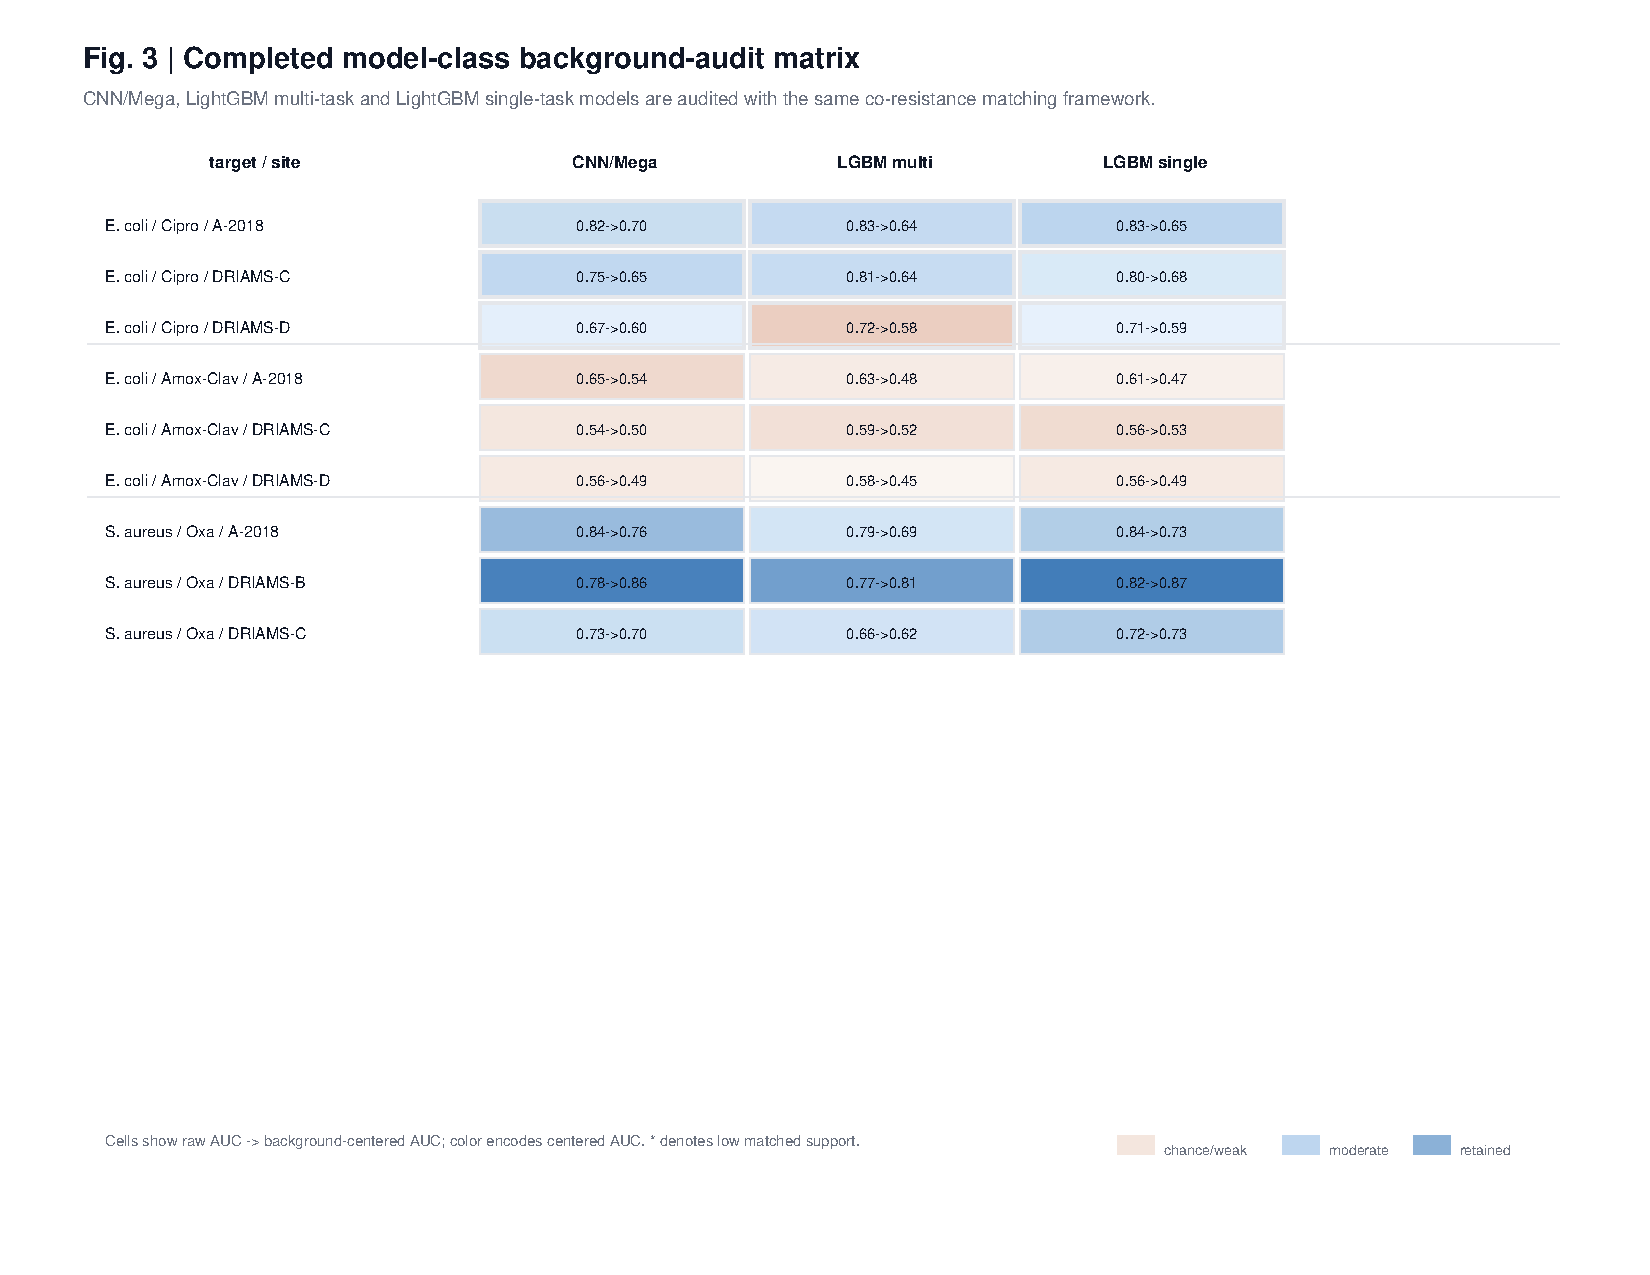
\includegraphics[width=\linewidth]{figures/figure_3_model_family_replication.pdf}
\caption{\textbf{Model-family replication.} The same background-matched audit is applied to CNN and multi-task LightGBM predictions. Both models show attenuation after background centering, with stronger residual signal for ciprofloxacin than amoxicillin-clavulanic acid across the primary interpretable sites.}
\label{fig:model-replication}
\end{figure}

\begin{table}[ht]
\centering
\small
\caption{Model-family audit of raw-to-background-centered attenuation.}
\label{tab:model-replication}
\resizebox{\linewidth}{!}{%
\begin{tabular}{lcccccc}
\toprule
Model & Site & Drug & Raw AUC & Centered AUC & Retention & Adequacy \\
\midrule
Mega CNN & A-2018 & Amox-Clav & 0.650 & 0.541 & 0.922 & interpretable \\
LGBM multi & A-2018 & Amox-Clav & 0.635 & 0.482 & 0.922 & interpretable \\
Mega CNN & A-2018 & Cipro & 0.823 & 0.703 & 0.619 & interpretable \\
LGBM multi & A-2018 & Cipro & 0.828 & 0.640 & 0.619 & interpretable \\
Mega CNN & DRIAMS-C & Amox-Clav & 0.535 & 0.497 & 0.892 & interpretable \\
LGBM multi & DRIAMS-C & Amox-Clav & 0.593 & 0.518 & 0.892 & interpretable \\
Mega CNN & DRIAMS-C & Cipro & 0.750 & 0.646 & 0.476 & interpretable \\
LGBM multi & DRIAMS-C & Cipro & 0.814 & 0.637 & 0.476 & interpretable \\
Mega CNN & DRIAMS-D & Amox-Clav & 0.557 & 0.486 & 0.974 & interpretable \\
LGBM multi & DRIAMS-D & Amox-Clav & 0.580 & 0.449 & 0.974 & interpretable \\
Mega CNN & DRIAMS-D & Cipro & 0.671 & 0.596 & 0.984 & interpretable \\
LGBM multi & DRIAMS-D & Cipro & 0.723 & 0.576 & 0.984 & interpretable \\
Weis/Borgwardt-style logistic regression & DRIAMS-C & Amox-Clav & 0.626 & 0.578 & 0.746 & interpretable \\
Weis/Borgwardt-style logistic regression & DRIAMS-C & Cipro & 0.625 & 0.816 & 0.438 & caution\_low\_n\_matched \\
Weis/Borgwardt-style logistic regression & DRIAMS-D & Amox-Clav & 0.652 & 0.524 & 0.925 & interpretable \\
Weis/Borgwardt-style logistic regression & DRIAMS-D & Cipro & 0.667 & 0.620 & 0.915 & interpretable \\
\bottomrule
\end{tabular}%
}
\vspace{2mm}\parbox{0.95\linewidth}{\footnotesize The same audit is applied to Mega/CNN, multi-task LGBM and a Weis/Borgwardt-style compatibility export. Weis rows are supplementary and are not claimed as an exact replication of Weis et al.}
\end{table}


\subsection*{Resistance labels form strong co-resistance blocks}

The audit depends on a biological premise: resistant labels are not independent. We therefore built a cross-resistance network from isolate-level AST labels. The strongest edge was ciprofloxacin/norfloxacin (phi=0.976; resistant Jaccard=0.963), showing that these two fluoroquinolones largely identify the same resistant subpopulation. The next strongest edges were among third- and fourth-generation cephalosporins: ceftriaxone/ceftazidime (phi=0.884), ceftazidime/cefepime (phi=0.828) and ceftriaxone/cefepime (phi=0.804) (Fig.~\ref{fig:cross-resistance}; Table~\ref{tab:cross-resistance}).

\begin{figure}[ht]
\centering
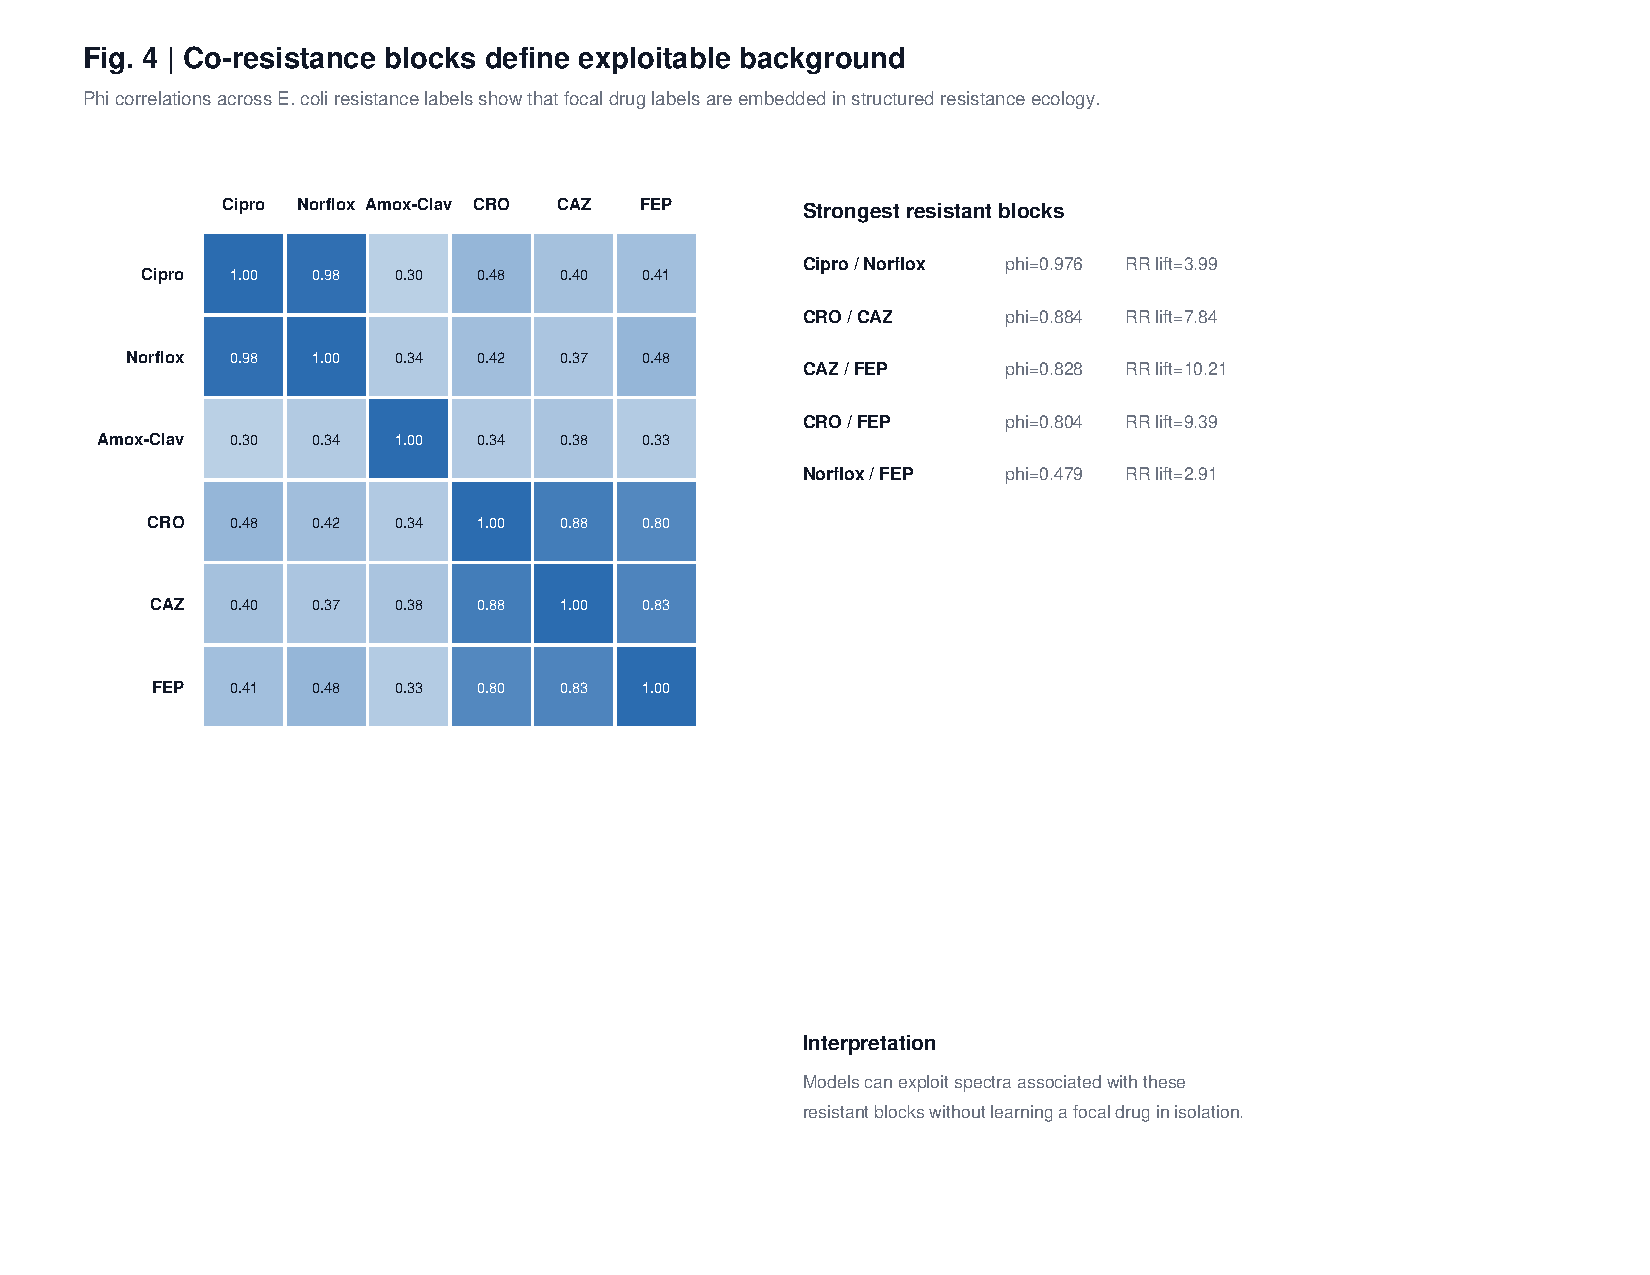
\includegraphics[width=\linewidth]{figures/figure_4_cross_resistance_network.pdf}
\caption{\textbf{Cross-resistance network in the expanded \textit{E. coli} panel.} Pairwise phi correlations show strong fluoroquinolone and cephalosporin resistance blocks. These blocks are the ecological structures that a MALDI-TOF AMR model can exploit if spectral background co-segregates with resistance labels.}
\label{fig:cross-resistance}
\end{figure}

\begin{table}[ht]
\centering
\small
\caption{Strongest co-resistance edges in the E. coli expanded panel.}
\label{tab:cross-resistance}
\resizebox{\linewidth}{!}{%
\begin{tabular}{lcccccc}
\toprule
Drug A & Drug B & n both & n RR & RR lift & Phi & R Jaccard \\
\midrule
Cipro & Norflox & 1090 & 263 & 3.993 & 0.976 & 0.963 \\
CRO & CAZ & 4349 & 446 & 7.841 & 0.884 & 0.811 \\
CAZ & FEP & 3907 & 271 & 10.212 & 0.828 & 0.719 \\
CRO & FEP & 3956 & 283 & 9.394 & 0.804 & 0.680 \\
Norflox & FEP & 771 & 89 & 2.908 & 0.479 & 0.392 \\
Cipro & CRO & 4371 & 437 & 3.223 & 0.479 & 0.382 \\
\bottomrule
\end{tabular}%
}
\vspace{2mm}\parbox{0.95\linewidth}{\footnotesize Edges are computed across isolate-level AST labels. RR lift compares observed double resistance with the expectation under independence.}
\end{table}


This network explains why raw AUC alone is insufficient. A model trained to predict cefepime resistance may exploit spectral features associated with a broader cephalosporin-resistant background. Such a model can still be clinically useful, but the interpretation differs from focal cefepime biology. Background-centered AUC quantifies how much ranking remains after that background is controlled.

\subsection*{Public WGS-linked MALDI data support strong lineage encoding}

The background-matched audit is designed for datasets without WGS labels. To test whether the underlying biological concern is plausible, we used an independent public Basel/Cuenod uropathogenic \textit{E. coli} resource that links WGS-derived metadata and Bruker MALDI peak features. After joining public metadata and Bruker median-peak tables, 407 isolates had usable peak features; 55 were ST131. A simple centroid-direction classifier predicted ST131 lineage from MALDI peak features with AUC 0.906, whereas ciprofloxacin and ceftriaxone resistance were predicted with AUCs 0.739 and 0.650 (Fig.~\ref{fig:public-support}a; Table~\ref{tab:public-wgs}).

We then asked whether discriminative MALDI peak bins for ST131 and resistance phenotypes were enriched for published ST131 MALDI biomarker masses\cite{nakamura2019st131}. Among the top 75 bins per target, overlaps with published ST131 biomarkers were enriched beyond a mass-stratified permutation null: 14 overlaps for ST131 (3.11-fold, empirical p=0.0001), 10 for ciprofloxacin resistance (2.24-fold, p=0.0068), and 12 for ceftriaxone resistance (2.64-fold, p=0.0006) (Fig.~\ref{fig:public-support}b; Table~\ref{tab:biomarker-enrichment}).

\begin{figure}[ht]
\centering
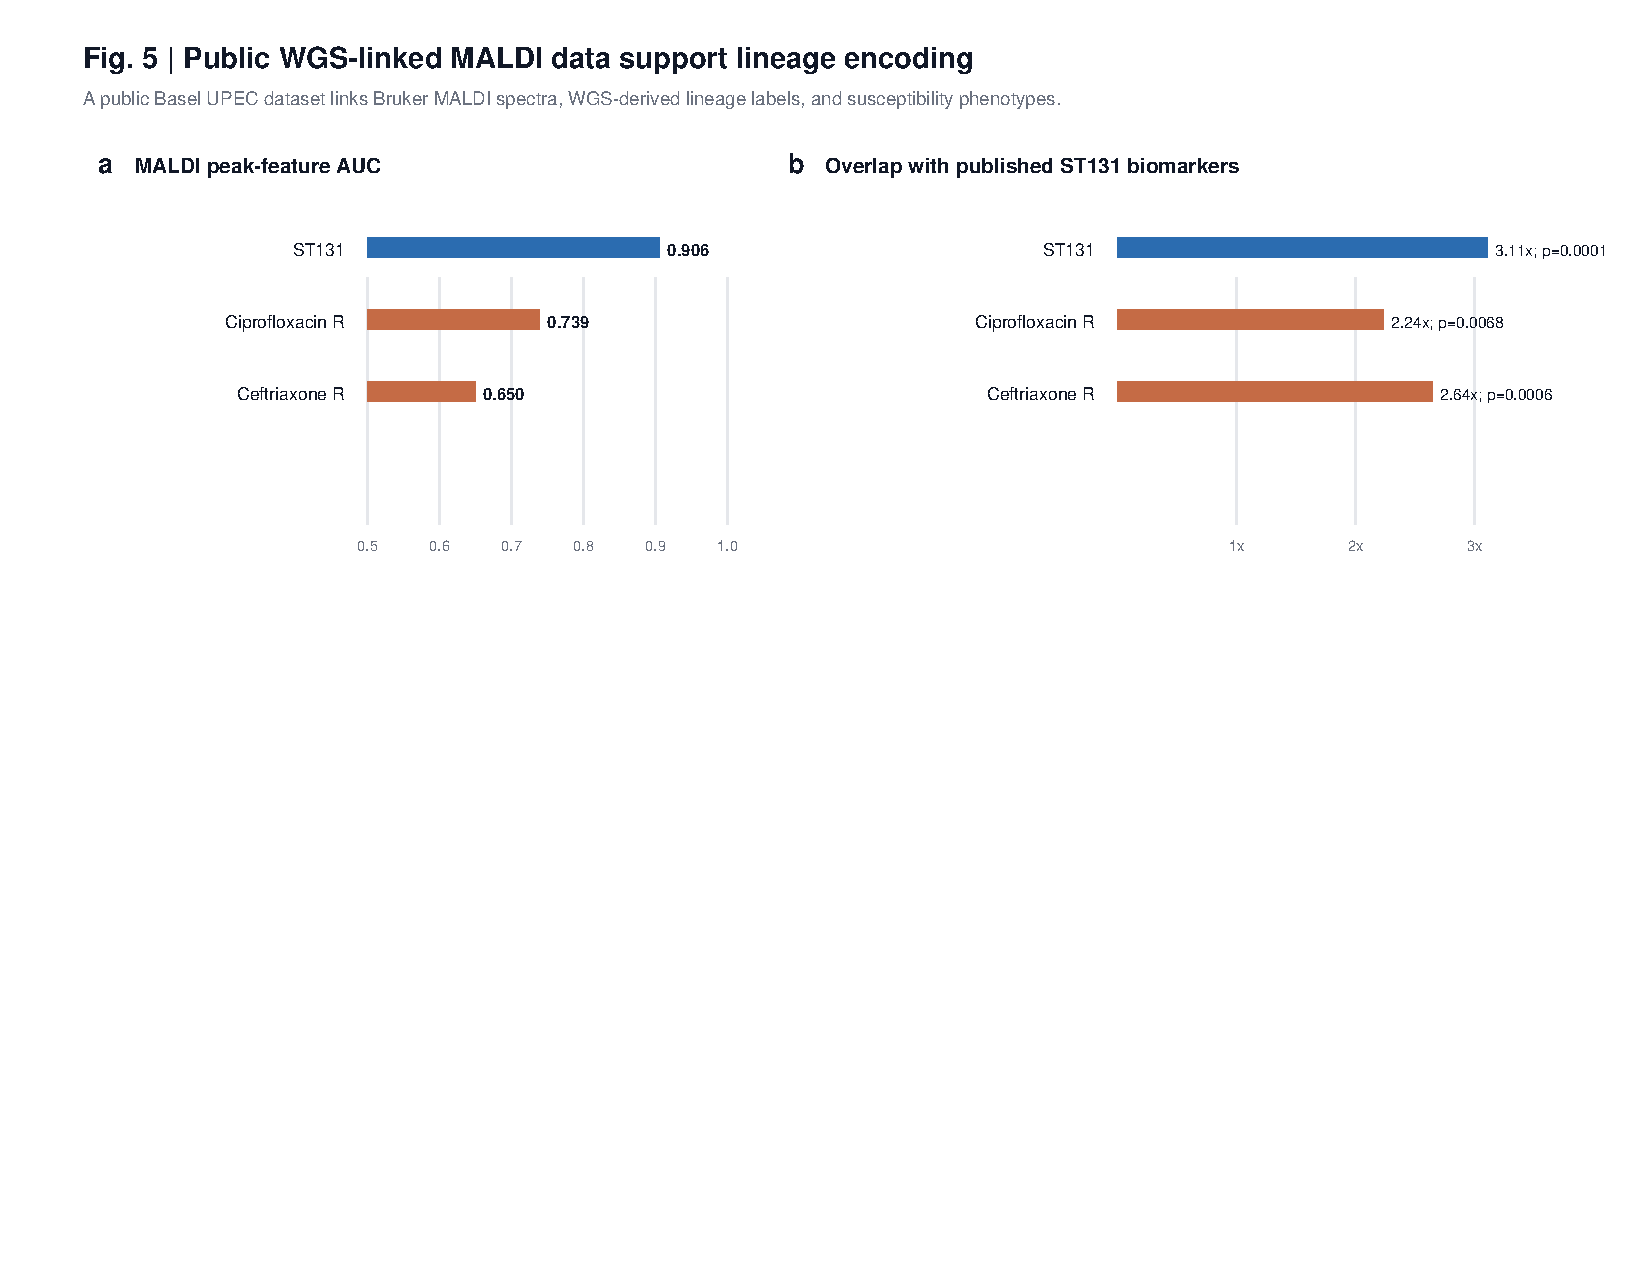
\includegraphics[width=\linewidth]{figures/figure_5_public_wgs_proteomic_support.pdf}
\caption{\textbf{Public WGS-linked Bruker data support lineage-associated MALDI signal.} \textbf{a}, ST131 lineage is more strongly encoded in public UPEC MALDI peak features than ciprofloxacin or ceftriaxone resistance. \textbf{b}, Discriminative peak bins are enriched for published ST131 MALDI biomarker masses under a mass-stratified permutation null.}
\label{fig:public-support}
\end{figure}

\begin{table}[ht]
\centering
\small
\caption{Public WGS-linked Basel UPEC MALDI validation.}
\label{tab:public-wgs}
\resizebox{\linewidth}{!}{%
\begin{tabular}{lccccc}
\toprule
Target & n & positive & AUC & folds & Model \\
\midrule
ST131 & 407 & 55 & 0.906 & 5 & centroid\_direction \\
Ciprofloxacin R & 350 & 53 & 0.739 & 5 & centroid\_direction \\
Ceftriaxone R & 360 & 30 & 0.650 & 5 & centroid\_direction \\
\bottomrule
\end{tabular}%
}
\vspace{2mm}\parbox{0.95\linewidth}{\footnotesize A simple centroid-direction classifier is used to ask whether lineage and resistance labels are encoded in Bruker MALDI peak features.}
\end{table}

\begin{table}[ht]
\centering
\small
\caption{Mass-neighborhood enrichment of published ST131 MALDI biomarkers among discriminative public UPEC peaks.}
\label{tab:biomarker-enrichment}
\resizebox{\linewidth}{!}{%
\begin{tabular}{lcccccccc}
\toprule
Target & Observed & $\leq$10 Da & 10--25 Da & $>$25 Da & Top peaks & Null mean & Fold enrichment & P perm \\
\midrule
ST131 & 14 & 4 & 7 & 3 & 75 & 4.51 & 3.11 & 0.0001 \\
Ciprofloxacin R & 10 & 3 & 4 & 3 & 75 & 4.47 & 2.24 & 0.0068 \\
Ceftriaxone R & 12 & 2 & 4 & 6 & 75 & 4.54 & 2.64 & 0.0006 \\
ALL TARGETS & 36 & 9 & 15 & 12 & 225 & 13.55 & 2.66 & 0.0001 \\
\bottomrule
\end{tabular}%
}
\vspace{2mm}\parbox{0.95\linewidth}{\footnotesize Observed overlaps are broad mass-neighborhood overlaps used for enrichment testing, not protein identifications. Matches $\leq$10\,Da are high-confidence mass correspondences, 10--25\,Da are putative, and $>$25\,Da are loose neighborhood overlaps listed for completeness only. The null model preserves the coarse m/z-stratum distribution of selected peaks.}
\end{table}


These public analyses are supporting evidence, not direct proof that the DRIAMS CNN detects ST131. They show that MALDI spectra can encode lineage strongly and that resistance-associated peak bins can overlap lineage-associated MALDI biomarkers. This is exactly the situation in which background-aware evaluation is needed before interpreting resistance prediction as focal resistance biology.

\subsection*{Guardrails for interpretation}

The framework intentionally separates supported claims from claims that would require WGS-linked DRIAMS isolates or direct proteomics. We can say that MALDI-TOF AMR models are background-sensitive, that raw AUC can overstate focal-drug signal, and that public WGS-linked spectra encode lineage strongly. We do not claim that every MALDI-TOF AMR prediction is clonal confounding, that DRIAMS predictions are definitively ST131 detection, or that the exact proteins behind discriminative peaks are identified. The reusable guardrail table is provided in the manuscript table folder for use as Supplementary Table 1.

\section*{Discussion}

This study reframes MALDI-TOF AMR evaluation from a performance-only question to a background-aware question. A model may have useful raw AUC while drawing part of its signal from the resistant bacterial population rather than the focal drug alone. The Background-Matched MALDI-AMR Audit supplies a practical test: does the model still rank resistant above susceptible isolates after controlling for co-resistance background?

The strongest evidence is the \textit{E. coli} ciprofloxacin versus amoxicillin-clavulanic acid contrast. Ciprofloxacin retains more residual signal after matching, whereas amoxicillin-clavulanic acid weakens or collapses toward chance at external sites with high matched retention. This does not prove a single mechanism. Rather, it supports a model in which MALDI-TOF AMR predictions are mixtures of focal physiology, lineage, co-resistance and hospital ecology. The contribution is to make that mixture measurable with ordinary isolate-level predictions and AST labels.

The public WGS-linked UPEC analysis gives independent biological grounding. In that dataset, MALDI peak features predict ST131 lineage more strongly than ciprofloxacin or ceftriaxone resistance, and resistance-associated discriminative peaks are enriched for published ST131 biomarker masses. This supports the plausibility that MALDI-TOF AMR models can use lineage-associated spectral structure. However, the public UPEC dataset is not a full second external deployment validation of the DRIAMS-trained model. It is a lineage-aware support analysis.

The framework also changes how negative or mixed results should be read. A low background-centered AUC does not mean MALDI-TOF AMR is useless. It means that raw performance may depend on background structure that could shift across hospitals. Conversely, retained centered AUC does not prove direct detection of a resistance protein. It means that the model contains residual ranking signal inside matched backgrounds. These distinctions are essential for clinical deployment, because a hospital deploying a model needs to know whether its local resistant subpopulation resembles the training population.

This study has limitations. Co-resistance background is an imperfect proxy for phylogeny and mobile genetic context. WGS or MLST labels linked to DRIAMS isolates would provide a stronger test of clone-versus-focal signal. Saliency and biomarker overlap analyses are supportive but cannot identify proteins without MS/MS, MALDI-TOF/TOF, LC-MS/MS or comparable validation. Some organism-drug-site pairs have low matched retention and should be flagged rather than overinterpreted. Finally, the Weis-style audit is currently best treated as a compatibility and supplementary analysis unless rerun with locked full-row prediction exports.

The practical recommendation is simple: MALDI-TOF AMR papers and deployments should report more than raw AUC. They should report whether predictions survive background matching, how much data remain interpretable, and which co-resistance blocks exist in the target population. This makes the interpretation of performance more honest and improves the chance that models will be evaluated on the signal they are expected to carry in clinical practice.

\section*{Methods}

\subsection*{DRIAMS datasets and organism-drug panels}

We used DRIAMS MALDI-TOF spectra and AST labels as the primary clinical benchmark\cite{weis2022driams,driamsdryad}. Models were trained on DRIAMS-A pre-2018 isolates and evaluated on a temporal DRIAMS-A 2018 split and external DRIAMS-B, DRIAMS-C and DRIAMS-D sites. The expanded \textit{E. coli} panel used ciprofloxacin, norfloxacin, amoxicillin-clavulanic acid, ceftriaxone, ceftazidime and cefepime. Intermediate or unavailable AST calls were treated as missing for the corresponding binary focal-drug comparison.

\subsection*{Prediction models}

The main neural model was the repository's multi-task CNN/Mega model trained from MALDI-TOF spectra with a 2,000--20,000 m/z representation. LightGBM baselines were trained from the same data splits and audited with the same model-agnostic pipeline. The goal of the LightGBM comparison was not to tune a superior baseline, but to test whether background sensitivity persisted outside the CNN architecture.

\subsection*{Background signatures}

For each isolate and focal drug, a background signature was constructed from the AST calls of the non-focal drugs in the same organism panel. Resistant calls were encoded as R, susceptible calls as S and unavailable calls as U. For example, when auditing ciprofloxacin, norfloxacin and beta-lactam labels contribute to the co-resistance background signature, while ciprofloxacin itself is excluded. The default audit retained strata with at least three resistant and three susceptible isolates for the focal drug. Sensitivity analyses using minimum thresholds of two, three and five isolates per class are implemented in the software.

\subsection*{Background-centered AUC}

For each site, organism and focal drug, raw AUC was computed from all available prediction rows. Matched AUC was computed after restricting to valid co-resistance strata. For background-centered AUC, each prediction score was centered by subtracting the mean score within its valid background stratum. AUC was then recomputed from the centered scores. This statistic is stricter than matched AUC because it removes stratum-level score shifts shared by resistant and susceptible isolates within the same background.

\subsection*{Pairwise within-background accuracy}

For each valid background stratum, every resistant isolate was paired with every susceptible isolate for the focal drug. A within-background pair was counted as correct if the resistant isolate had the higher model score, half-correct if tied and incorrect otherwise. Pairwise within-background accuracy is the average over all such pairs. This metric is equivalent in spirit to AUC restricted to matched backgrounds, but it is reported separately because it makes the number of within-background comparisons explicit.

\subsection*{Uncertainty and permutation testing}

Bootstrap confidence intervals were computed by resampling prediction rows with replacement. Permutation p values were computed by shuffling focal-drug labels within valid background strata and recomputing centered AUC. The default audit used 500 bootstrap replicates and 500 permutations. Low-support rows were labeled using adequacy thresholds for matched sample count, matched retention and pairwise comparisons.

\subsection*{Cross-resistance network}

Cross-resistance edges were computed from isolate-level AST labels. For each drug pair, we counted susceptible-susceptible, susceptible-resistant, resistant-susceptible and resistant-resistant combinations. We reported phi correlation, resistant-resistant lift relative to independence and resistant Jaccard similarity. These metrics quantify the co-resistance blocks that a MALDI-TOF model could exploit.

\subsection*{Public WGS-linked UPEC analysis}

We used public Basel/Cuenod uropathogenic \textit{E. coli} resources linking WGS metadata and Bruker MALDI-derived median peak features\cite{cuenod2023papgii}. Processed manifests in this repository join ENA accessions, OSF Bruker files and metadata from the public project. We built binned MALDI peak features from Bruker median peaks and evaluated a centroid-direction classifier for ST131, ciprofloxacin resistance and ceftriaxone resistance using five folds. This analysis tests whether lineage and resistance phenotypes are encoded in public MALDI peak features; it is not a deployment test of the DRIAMS-trained CNN.

\subsection*{Published ST131 biomarker enrichment}

Published ST131 MALDI biomarker masses were taken from the Scientific Reports proteomic analysis of ESBL-producing \textit{E. coli} ST131\cite{nakamura2019st131}. For ST131, ciprofloxacin resistance and ceftriaxone resistance in the public UPEC dataset, we ranked MALDI bins by the absolute difference in mean log-intensity between positive and negative isolates. The top 75 bins per target were compared with the published ST131 biomarker list using a 40 Da tolerance. A mass-stratified permutation null sampled the same number of peak bins with the same coarse m/z-stratum distribution and counted overlaps with the biomarker list. This analysis identifies non-random overlap with published biomarker masses; it does not identify proteins de novo.

\subsection*{Software and reproducibility}

All analyses are organized around a model-agnostic prediction table. Any model can be audited if it exports isolate identifier, site, year, organism, drug, binary AST label and model probability. The main audit script is \texttt{run\_background\_audit\_framework.py}. Publication figures and LaTeX tables are generated by \texttt{scripts/make\_ncomms\_figures.py}.

\section*{Data availability}

Raw DRIAMS spectra and AST files are not redistributed in this repository and should be obtained from the official DRIAMS release\cite{driamsdryad}. Public UPEC WGS and MALDI resources are available from ENA project PRJEB55855, ENA study ERP140793, the Cu{\'e}nod UPEC GitHub repository and the associated OSF project. This repository includes processed manifests and derived summary outputs used to regenerate the manuscript figures.

\section*{Code availability}

The analysis code is available at \url{https://github.com/byungkim113/background-matched-maldi-amr-audit}. The repository includes the model-agnostic audit engine, prediction exporters, public UPEC WGS/proteomic support analyses, figure-generation code and reproducibility documentation.

\section*{Acknowledgements}

We thank the DRIAMS, MALDI-AMR and public UPEC data generators for releasing resources that make external benchmarking and background-aware reanalysis possible.

\section*{Author contributions}

B.K. conceived the background-matched audit, implemented analyses, generated figures and wrote the initial manuscript draft. Additional author contributions should be completed before submission.

\section*{Competing interests}

The authors declare no competing interests. This statement should be confirmed by all authors before submission.

\section*{Additional information}

Correspondence and requests for materials should be addressed to the corresponding author.

\begin{thebibliography}{10}

\bibitem{weis2022driams}
Weis, C. \textit{et al.} Direct antimicrobial resistance prediction from clinical MALDI-TOF mass spectra using machine learning. \textit{Nat. Med.} \textbf{28}, 164--174 (2022).

\bibitem{driamsdryad}
Weis, C. \textit{et al.} DRIAMS: Database of Resistance Information on Antimicrobials and Mass Spectra. Dryad. \url{https://doi.org/10.5061/dryad.bzkh1899q} (2022).

\bibitem{yu2025population}
Yu, Y., Wheeler, N. E. \& Barquist, L. Biased sampling driven by bacterial population structure confounds machine learning prediction of antimicrobial resistance. \textit{PLOS Biol.} \textbf{23}, e3003539 (2025).

\bibitem{weis2022stratification}
Weis, C., Rieck, B. A., Balzer, S., Cu{\'e}nod, A., Egli, A. \& Borgwardt, K. Improved MALDI-TOF MS based antimicrobial resistance prediction through hierarchical stratification. \textit{bioRxiv} \url{https://doi.org/10.1101/2022.04.13.488198} (2022).

\bibitem{cuenod2023papgii}
Cu{\'e}nod, A. \textit{et al.} Bacterial genome-wide association study substantiates papGII of \textit{Escherichia coli} as a major risk factor for urosepsis. \textit{Genome Med.} \textbf{15}, 89 (2023).

\bibitem{nicolas2014st131}
Nicolas-Chanoine, M.-H., Bertrand, X. \& Madec, J.-Y. \textit{Escherichia coli} ST131, an intriguing clonal group. \textit{Clin. Microbiol. Rev.} \textbf{27}, 543--574 (2014).

\bibitem{nakamura2019st131}
Nakamura, A. \textit{et al.} Identification of specific protein amino acid substitutions of extended-spectrum beta-lactamase-producing \textit{Escherichia coli} ST131: a proteomics approach using mass spectrometry. \textit{Sci. Rep.} \textbf{9}, 8555 (2019).

\end{thebibliography}

\end{document}
